%\graphicspath{anexos/recursos/}
\section{Descripción detallada de los casos de prueba} \label{Anexo:tabla-casos}

Nótese que se ha saltado el caso 2. Esto se debe a que el correspondiente caso 2 enviado por \gls{CRIDA} tenía una falta de datos que impedía su uso. Se ha decidido mantener la misma nomenclatura para una concordancia total con el código entregado.





\subsection{Caso 1}

\textbf{Unidad de Control}: Barcelona

\textbf{Incidencia}: Modificación de sectorizaciones. La \autoref{fig:5:caso1} muestra cómo es este cambio.
Como podemos ver...



%\begin{table}[h]
%	\begin{tabular}{|c|c|c|}
%		\hline
%		          \textbf{Núcleo}            & \textbf{Sectorización} & \textbf{Intervalo} \\ \hline
%		\multirow{2}{*}{Barcelona Ruta Este} &           3D           & 7:30:00--15:00:00  \\ \cline{2-3}
%		                                     &           5A           & 7:30:00--10:30:00  \\ \hline
%		        Barcelona Ruta Oeste         &           6C           & 10:30:00--15:00:00 \\ \hline
%	\end{tabular}
%\end{table}
\begin{table}[h]
	\centering
	\caption{Sectorización modificada del Caso 1}
	\begin{tabular}{ccc}
		\hline
		\textbf{Núcleo}                                           & \textbf{Configuración} & \textbf{Intervalo}   \\ \hline
		\multicolumn{1}{l}{}                                      & \multicolumn{1}{l}{}   & \multicolumn{1}{l}{} \\
		\multicolumn{1}{c|}{\multirow{2}{*}{Barcelona Ruta Este}} & 3D                     & 7:30:00--15:00:00    \\
		\multicolumn{1}{c|}{}                                     & 5A                     & 7:30:00--10:30:00    \\
		\multicolumn{1}{l}{}                                      & \multicolumn{1}{l}{}   & \multicolumn{1}{l}{} \\
		Barcelona Ruta Oeste                                      & 6C                     & 10:30:00--15:00:00   \\ \hline
	\end{tabular}
	\label{table:5:caso1-modif}
\end{table}


\subsection{Caso 3}\footnote{Nótese que se ha saltado el caso 2. Esto se debe a que el correspondiente caso 2 enviado por \gls{CRIDA} tenía una falta de datos que impedía su uso. Se ha decidido mantener la misma nomenclatura para una concordancia total con el código entregado.}

\textbf{Unidad de Control}: Barcelona

\textbf{Situación inicial}:
\begin{itemize}[label={}]
	
	\item \textbf{Turno}: MC, 7:30-15:00
	
	\item \textbf{Recursos}: \\
	7 PTD Barcelona Ruta Este \\
	17 PTD Barcelona Ruta Oeste
	
	
	\item \textbf{Sectorización}: véase la \autoref{table:5:caso3-inicial}
	\begin{table}[h]
		\centering
		\caption{Sectorización inicial del Caso 1}
		\begin{tabular}{ccc}
			\hline
			\textbf{Núcleo}      & \textbf{Configuración} & \textbf{Intervalo}   \\ \hline
			\multicolumn{1}{l}{} & \multicolumn{1}{l}{}   & \multicolumn{1}{l}{} \\
			Barcelona Ruta Este  & 3D                     & 7:30:00--15:00:00    \\
			\multicolumn{1}{l}{} & \multicolumn{1}{l}{}   & \multicolumn{1}{l}{} \\
			Barcelona Ruta Oeste & 5A                     & 10:30:00--15:00:00   \\ \hline
		\end{tabular}
		\label{table:5:caso3-inicial}
	\end{table}
	
	
\end{itemize}

\textbf{Momento del Cambio}: 10:00:00

\textbf{Tipo incidencia}: Baja de un controlador

\textbf{Descripción}:Se produce una baja del controlador $c_{23}$ a las 9:30. No se producen altas. Se necesita 1 controlador imaginarios para inicializar este caso.

\subsection{Caso 4}

\textbf{Unidad de Control}: Madrid

\textbf{Situación inicial}:
\begin{itemize}[label={}]
	
	\item \textbf{Turno}: MC, 7:30-15:00
	
	\item \textbf{Recursos}: \\
	7 PTD Barcelona Ruta Este \\
	17 PTD Barcelona Ruta Oeste
	
	
	\item \textbf{Sectorización}: véase la \autoref{table:5:caso1-inicial}
	\begin{table}[h]
		\centering
		\caption{Sectorización inicial del Caso 1}
		\begin{tabular}{ccc}
			\hline
			\textbf{Núcleo}      & \textbf{Configuración} & \textbf{Intervalo}   \\ \hline
			\multicolumn{1}{l}{} & \multicolumn{1}{l}{}   & \multicolumn{1}{l}{} \\
			Barcelona Ruta Este  & 3D                     & 7:30:00--15:00:00    \\
			\multicolumn{1}{l}{} & \multicolumn{1}{l}{}   & \multicolumn{1}{l}{} \\
			Barcelona Ruta Oeste & 5A                     & 10:30:00--15:00:00   \\ \hline
		\end{tabular}
		\label{table:5:caso1-inicial}
	\end{table}
	
	
\end{itemize}

\textbf{Momento del Cambio}: 10:00:00

\textbf{Tipo incidencia}: Modificación de sectorizaciones

\textbf{Descripción}:Pasamos de una 3D a una 5A, lo que implica el cierre de un sector y la apertura de otros dos. Además se abre un sector adicional en el núcleo \textit{Barcelona Ruta Oeste}. La nueva sectorización es la de la \autoref{table:5:caso1-modif}. Se necesitan 3 controladores imaginarios para inicializar éste caso.

%\begin{table}[h]
%	\begin{tabular}{|c|c|c|}
%		\hline
%		          \textbf{Núcleo}            & \textbf{Sectorización} & \textbf{Intervalo} \\ \hline
%		\multirow{2}{*}{Barcelona Ruta Este} &           3D           & 7:30:00--15:00:00  \\ \cline{2-3}
%		                                     &           5A           & 7:30:00--10:30:00  \\ \hline
%		        Barcelona Ruta Oeste         &           6C           & 10:30:00--15:00:00 \\ \hline
%	\end{tabular}
%\end{table}
\begin{table}[h]
	\centering
	\caption{Sectorización modificada del Caso 1}
	\begin{tabular}{ccc}
		\hline
		\textbf{Núcleo}                                           & \textbf{Configuración} & \textbf{Intervalo}   \\ \hline
		\multicolumn{1}{l}{}                                      & \multicolumn{1}{l}{}   & \multicolumn{1}{l}{} \\
		\multicolumn{1}{c|}{\multirow{2}{*}{Barcelona Ruta Este}} & 3D                     & 7:30:00--15:00:00    \\
		\multicolumn{1}{c|}{}                                     & 5A                     & 7:30:00--10:30:00    \\
		\multicolumn{1}{l}{}                                      & \multicolumn{1}{l}{}   & \multicolumn{1}{l}{} \\
		Barcelona Ruta Oeste                                      & 6C                     & 10:30:00--15:00:00   \\ \hline
	\end{tabular}
	\label{table:5:caso1-modif}
\end{table}





% En caso de borrar esta línea, eliminar el paquete \usepackage{pdfpages}
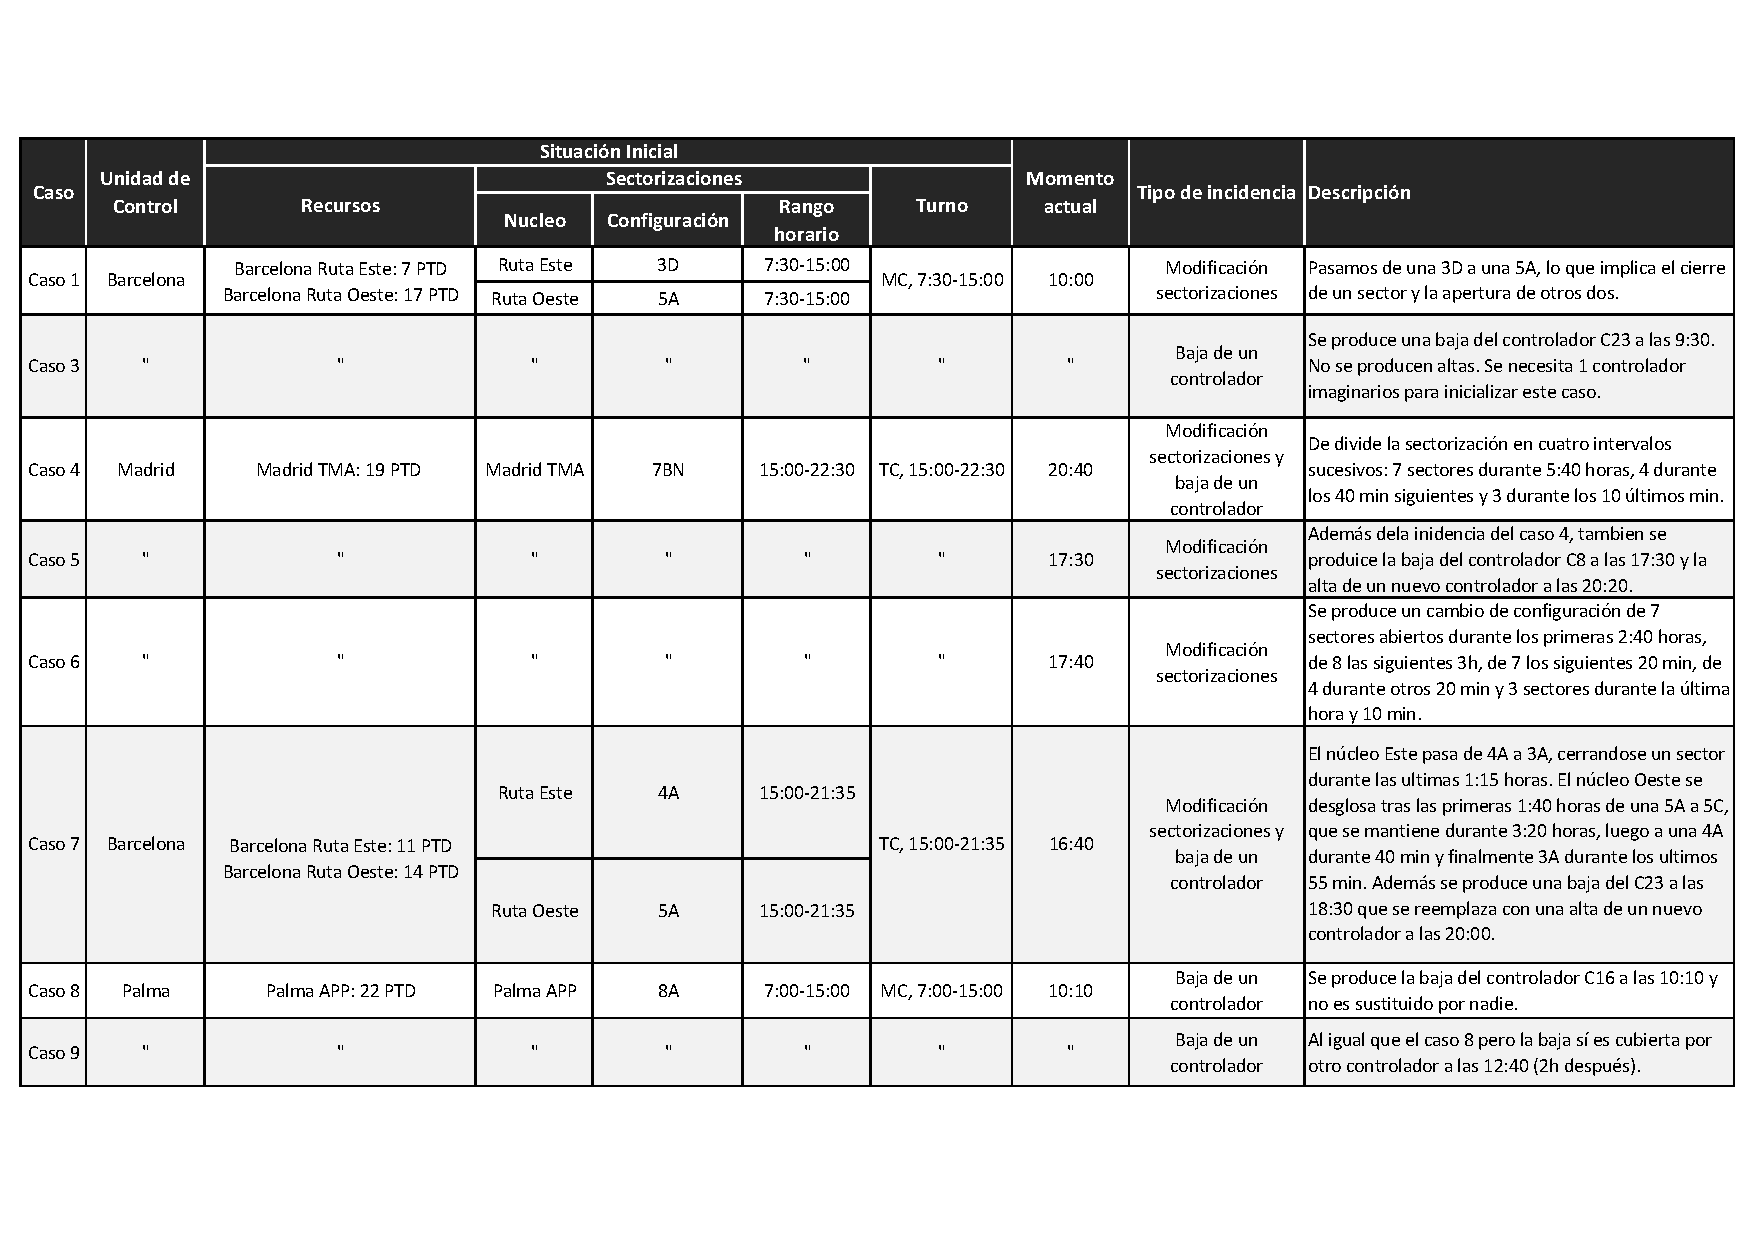
\includepdf[landscape=True]{tabla-casos}